%% Преамбула TeX-файла

% 1. Стиль и язык
\documentclass[utf8x, times, 14pt]{G7-32/tex/G7-32}

\setdefaultlanguage[babelshorthands=true]{russian}
% Остальные стандартные настройки убраны в preamble.inc.tex.
\sloppy

% Настройки стиля ГОСТ 7-32
% Для начала определяем, хотим мы или нет, чтобы рисунки и таблицы нумеровались в пределах раздела, или нам нужна сквозная нумерация.
\EqInChapter % формулы будут нумероваться в пределах раздела
\TableInChapter % таблицы будут нумероваться в пределах раздела
\PicInChapter % рисунки будут нумероваться в пределах раздела

% Добавляем гипертекстовое оглавление в PDF
\usepackage[
bookmarks=true, colorlinks=true, unicode=true,
urlcolor=black,linkcolor=black, anchorcolor=black,
citecolor=black, menucolor=black, filecolor=black,
]{hyperref}

\usepackage{pdfpages} % пакет для импорта pdf-файлов

\AfterHyperrefFix

\usepackage{microtype}% полезный пакет для микротипографии, увы под xelatex мало чего умеет, но под pdflatex хорошо улучшает читаемость

\usepackage{etoolbox}

\AtBeginEnvironment{minted}{%
  \setlength\abovecaptionskip{0pt}%
  \setlength\belowcaptionskip{0pt}%
}

% Тире могут быть невидимы в Adobe Reader
\ifInvisibleDashes
\MakeDashesBold
\fi

\usepackage{graphicx}   % Пакет для включения рисунков

% С такими оно полями оно работает по-умолчанию:
% \RequirePackage[left=20mm,right=10mm,top=20mm,bottom=20mm,headsep=0pt,includefoot]{geometry}
% Если вас тошнит от поля в 10мм --- увеличивайте до 20-ти, ну и про переплёт не забывайте:
\geometry{right=20mm}
\geometry{left=30mm}
\geometry{bottom=20mm}
\geometry{ignorefoot}% считать от нижней границы текста

\usepackage{svg}

% Пакет Tikz
\usepackage{tikz}
\usetikzlibrary{arrows,positioning,shadows}

% Произвольная нумерация списков.
\usepackage{enumerate}

% ячейки в несколько строчек
\usepackage{multirow}

% itemize внутри tabular
\usepackage{paralist,array}

%\setlength{\parskip}{1ex plus0.5ex minus0.5ex} % разрыв между абзацами
%\setlength{\parskip}{1ex} % разрыв между абзацами

% Центрирование подписей к плавающим окружениям
%\usepackage[justification=centering]{caption}

\usepackage{newfloat}
\DeclareFloatingEnvironment[
placement={!ht},
name=Equation
]{eqndescNoIndent}
\edef\fixEqndesc{\noexpand\setlength{\noexpand\parindent}{\the\parindent}\noexpand\setlength{\noexpand\parskip}{\the\parskip}}
\newenvironment{eqndesc}[1][!ht]{%
    \begin{eqndescNoIndent}[#1]%
\fixEqndesc%
}
{\end{eqndescNoIndent}}




% Настройки листингов.
\ifPDFTeX
% 8 Листинги

\usepackage{listings}

% Значения по умолчанию
\lstset{
  basicstyle=\normalsize,
  breakatwhitespace=true,% разрыв строк только на whitespacce
  breaklines=true,       % переносить длинные строки
%   captionpos=b,          % подписи снизу -- вроде не надо
  inputencoding=koi8-r,
  numbers=left,          % нумерация слева
  numberstyle=\normalsize,
  showspaces=false,      % показывать пробелы подчеркиваниями -- идиотизм 70-х годов
  showstringspaces=false,
  showtabs=false,        % и табы тоже
  stepnumber=1,
  tabsize=4,              % кому нужны табы по 8 символов?
  frame=single
}

% Стиль для псевдокода: строчки обычно короткие, поэтому размер шрифта побольше
\lstdefinestyle{pseudocode}{
  basicstyle=\normal,
  keywordstyle=\color{black}\bfseries\underbar,
  language=Pseudocode,
  numberstyle=\footnotesize,
  commentstyle=\footnotesize\it
}

% Стиль для обычного кода: маленький шрифт
\lstdefinestyle{realcode}{
  basicstyle=\scriptsize,
  numberstyle=\footnotesize
}

% Стиль для коротких кусков обычного кода: средний шрифт
\lstdefinestyle{simplecode}{
  basicstyle=\footnotesize,
  numberstyle=\footnotesize
}

% Стиль для BNF
\lstdefinestyle{grammar}{
  basicstyle=\footnotesize,
  numberstyle=\footnotesize,
  stringstyle=\bfseries\ttfamily,
  language=BNF
}

% Определим свой язык для написания псевдокодов на основе Python
\lstdefinelanguage[]{Pseudocode}[]{Python}{
  morekeywords={each,empty,wait,do},% ключевые слова добавлять сюда
  morecomment=[s]{\{}{\}},% комменты {а-ля Pascal} смотрятся нагляднее
  literate=% а сюда добавлять операторы, которые хотите отображать как мат. символы
    {->}{\ensuremath{$\rightarrow$}~}2%
    {<-}{\ensuremath{$\leftarrow$}~}2%
    {:=}{\ensuremath{$\leftarrow$}~}2%
    {<--}{\ensuremath{$\Longleftarrow$}~}2%
}[keywords,comments]

% Свой язык для задания грамматик в BNF
\lstdefinelanguage[]{BNF}[]{}{
  morekeywords={},
  morecomment=[s]{@}{@},
  morestring=[b]",%
  literate=%
    {->}{\ensuremath{$\rightarrow$}~}2%
    {*}{\ensuremath{$^*$}~}2%
    {+}{\ensuremath{$^+$}~}2%
    {|}{\ensuremath{$|$}~}2%
}[keywords,comments,strings]

% Подписи к листингам на русском языке.
\renewcommand\lstlistingname{Листинг}
\renewcommand\lstlistlistingname{Листинги}
\else
\usepackage{local-minted}
\fi

% Полезные макросы листингов.
% Любимые команды
\newcommand{\Code}[1]{\textbf{#1}}

\usepackage{enumitem}
% \setlist[itemize]{label=—, left=2.5em, nosep, topsep=0pt, partopsep=0pt}
\setlist[enumerate]{left=2.5em, labelwidth=2em, labelsep=0.25em, itemindent=3.75em, nosep, topsep=0pt, partopsep=0pt}
\setlist[itemize]{label=—, left=2.5em, labelwidth=2em, labelsep=0.25em, itemindent=3.75em, nosep, topsep=0pt, partopsep=0pt}

% Нумерация рисунков
\usepackage{caption}
\captionsetup[figure]{labelsep=endash, name=Рисунок}
\captionsetup[table]{labelsep=endash, name=Таблица}
\renewcommand{\thefigure}{\arabic{chapter}.\arabic{figure}}

\usepackage{titlesec}
\titleformat{\section}[hang]{\bfseries}{\hspace{1.25cm}\thesection}{1em}{}
\titleformat{\subsection}[hang]{\bfseries}{\hspace{1.25cm}\thesubsection}{1em}{}
\titleformat{\subsubsection}[hang]{\bfseries}{\hspace{1.25cm}\thesubsubsection}{1em}{}
\titleformat{name=\section,numberless}[hang]{\bfseries}{}{1em}{\centering}


% Перенос текста при переполнении
\emergencystretch=25pt


\titlespacing*{\chapter}{0pt}{0pt}{0pt}
\titlespacing*{\section}{0pt}{0pt}{0pt}
\titlespacing*{\subsection}{0pt}{0pt}{0pt}
\titlespacing*{\subsubsection}{0pt}{0pt}{0pt}

% Центрирование номера раздела
\renewcommand{\thechapter}{\arabic{chapter}.}
\renewcommand{\thesection}{\arabic{chapter}.\arabic{section}.}
\renewcommand{\thesubsection}{\arabic{chapter}.\arabic{section}.\arabic{subsection}.}
\renewcommand{\thesubsubsection}{\arabic{chapter}.\arabic{section}.\arabic{section}.\arabic{subsection}.}
\usepackage{setspace}

\makeatletter
\renewcommand{\@biblabel}[1]{#1)}
\makeatother

% Стиль титульного листа и заголовки

%\NirEkz{Экз. 3}                                  % Раскоментировать если не требуется
%\NirGrif{Секретно}                % Наименование грифа




\begin{document}

\frontmatter % выключает нумерацию ВСЕГО; здесь начинаются ненумерованные главы: реферат, введение, глоссарий, сокращения и прочее.

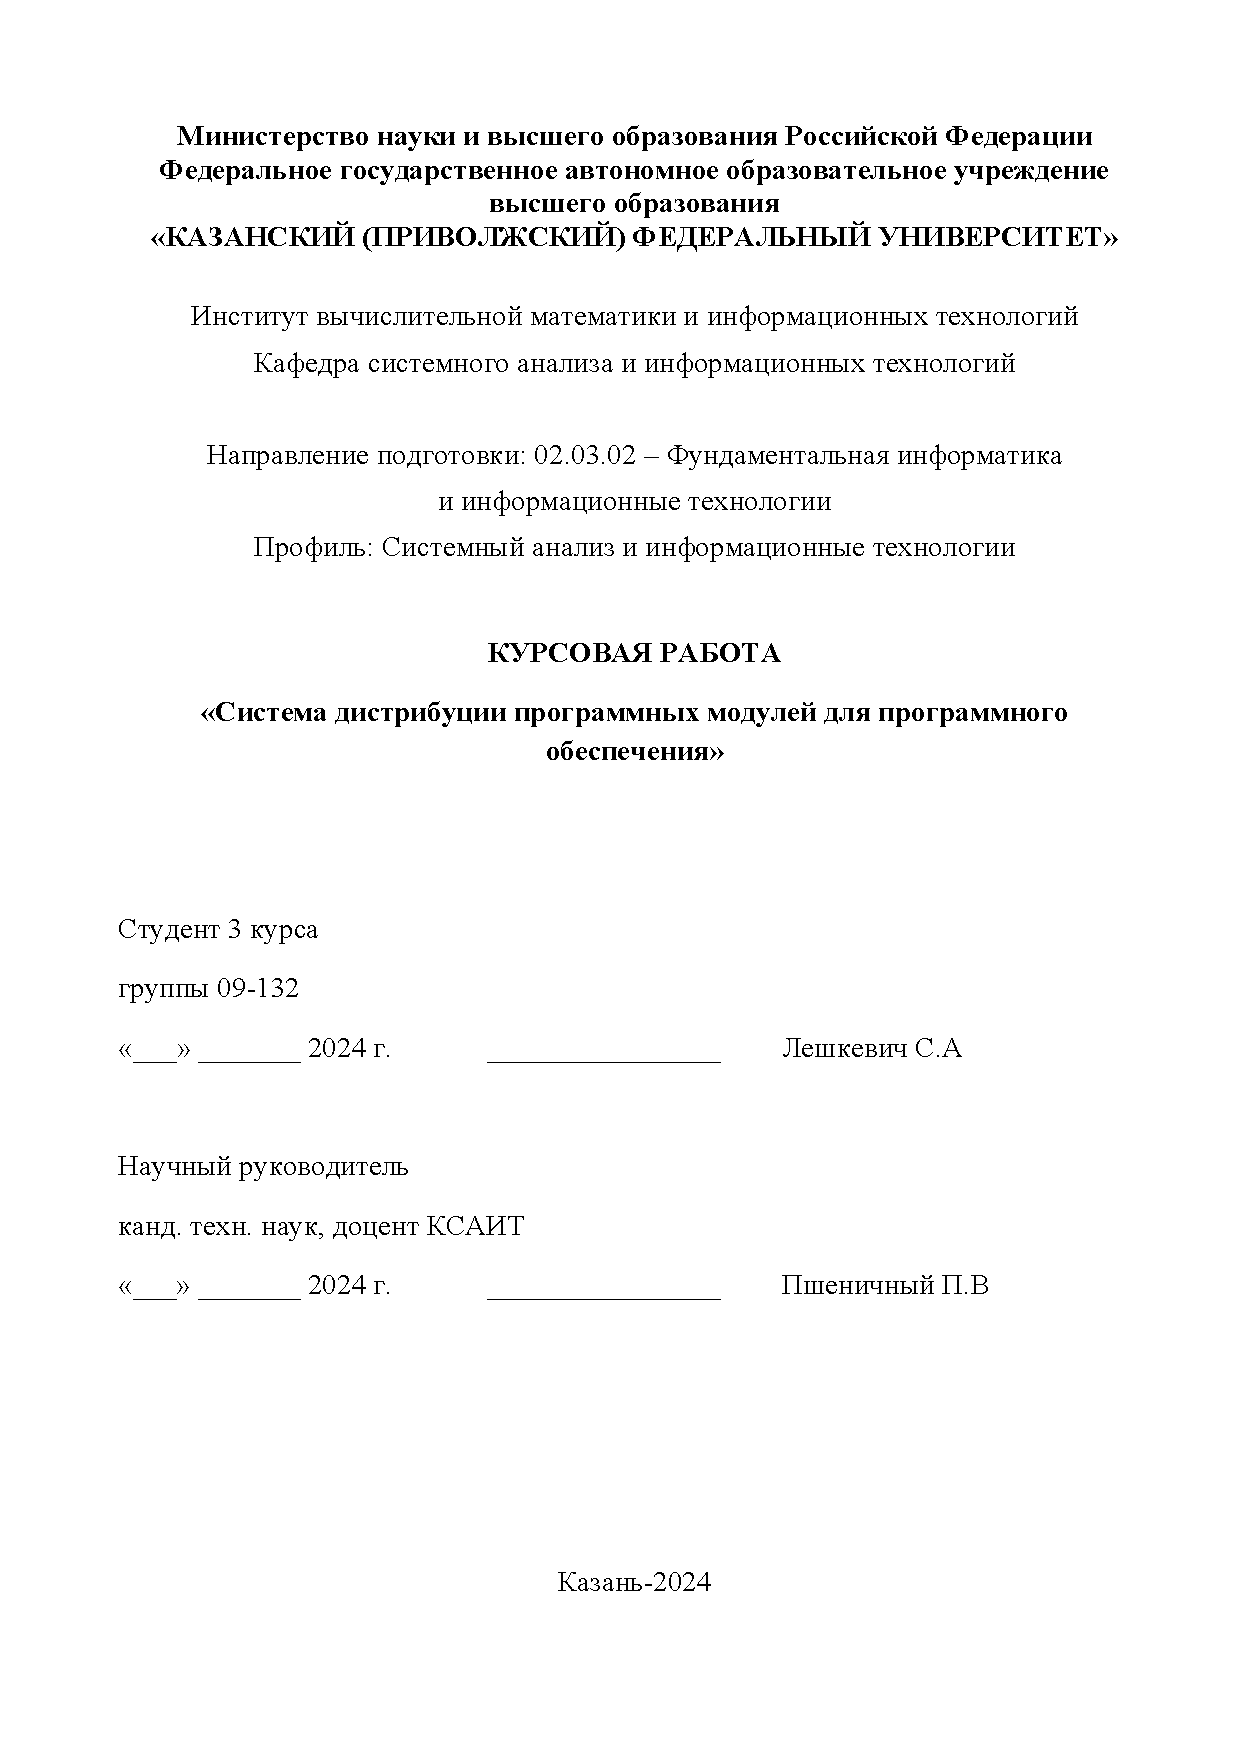
\includepdf[pages=-]{titlepage.pdf}


%\begin{executors}
%\personalSignature{Первый исполнитель}{ФИО}
%
%\personalSignature{Второй исполнитель}{ФИО}
%\end{executors}


%\listoffigures                         % Список рисунков

%\listoftables                          % Список таблиц

%\NormRefs % Нормативные ссылки 
% Команды \breakingbeforechapters и \nonbreakingbeforechapters
% управляют разрывом страницы перед главами.
% По-умолчанию страница разрывается.

% \nobreakingbeforechapters
% \breakingbeforechapters

%% Также можно использовать \Referat, как в оригинале
\begin{abstract}

    Отчет содержит \pageref{LastPage}\,стр.%
    \ifnum \totfig >0
    , \totfig~рис.%
    \fi
    \ifnum \tottab >0
    , \tottab~табл.%
    \fi
    %
    \ifnum \totbib >0
    , \totbib~источн.%
    \fi
    %
    \ifnum \totapp >0
    , \totapp~прил.%
    \else
    .%
    \fi


    Это пример каркаса расчётно-пояснительной записки, желательный к использованию в РПЗ проекта по курсу РСОИ
    \nocite{*}.

    Данный опус, как и более новые версии этого документа, можно взять по адресу (\url{https://github.com/latex-g7-32/latex-g7-32}).

    Текст в документе носит совершенно абстрактный характер.

\end{abstract}

%%% Local Variables: 
%%% mode: latex
%%% TeX-master: "rpz"
%%% End: 


\tableofcontents

\printnomenclature % Автоматический список сокращений

\Introduction

Работа над данной курсовой работой проходила на кафедре системного анализа и информационных технологий Института вычислительной математики и информационных технологий КФУ с 28 марта 2024 года по 24 мая 2024 года.
Целью данной практики была разработка системы дистрибуции программных модулей для программного обеспечения. Это необходимо для обеспечения удобства и эффективности работы с программным обеспечением, позволяет облегчить процесс обновления и масштабирования программного продукта. Данная система представляет из себя информационный ресурс, помогающий организовать и оптимизировать процесс дистрибуции программных модулей.

В рамках курсовой работы необходимо реализовать следующие задачи:

\renewcommand{\labelenumi}{\arabic{enumi})}
\renewcommand{\labelenumii}{\asbuk{enumii})}

\begin{enumerate}
\item Исследование и анализ предметной области,
\item Проектирование системы дистрибуции программных модулей,
\item Обзор и выбор технологий для разработки системы,
\item Разработка системы дистрибуции,
\item Проведение системного тестирования,
\item Анализ полученных результатов,
\item Оформление текста курсовой работы.
\end{enumerate}


\mainmatter % это включает нумерацию глав и секций в документе ниже

\chapter{  Исследование и анализ предметной области}

Для создания собственной системы дистрибуции необходимо изучить ее основные характеристики и ознакомиться с существующими на рынке решениями.

\section{Система дистрибуции модулей и ее смысл}

Система дистрибуции программных модулей — это набор инструментов и служб, предназначенный для управления разработкой, развертыванием, обновлением и управлением программными модулями (библиотеками, компонентами, пакетами или даже целыми программами) в программных проектах. Эти системы обычно используются для упрощения и автоматизации процесса управления зависимостями в программном обеспечении, а также для облегчения интеграции и совместимости различных модулей в больших и сложных системах.

Основные функции системы:

\begin{enumerate}
\item cоздание, удаление, обновление модуля;
\item управление зависимостями модулей;
\item версионность модулей;
\item информирование о модуляx;
\end{enumerate}

При этом система представляет собой ключевой инструмент в области разработки программного обеспечения, подстраивающийся под требования поддержки и разработки продукта. Позволяя обеспечивать бесперебойную работу продукта и его своевременное обновление, система дистрибуции вносит большой вклад в его адаптацию к меняющимся технологическим реалиям и потребностям пользователей.

Программные модули, будучи отдельными составляющими программного продукта с конкретными функциями или даже являясь полноценными программами, облегчают процесс разработки и предоставляют удобство в дальнейшем тестировании и сопровождении. Модульность также позволяет многократно использовать эти модули в разных частях программы, повышая эффективность в процессе разработки.

\section{Методы и способы организации систем дистрибуции}

Системы дистрибуции программных модулей, играя свою роль в увеличении эффективности разработки и обеспечении гарантии надежности работы, могут быть организованы разными способами. Эти способы варьируются от простых, таких как ручное копирование, до автоматических систем, которые включают механизмы контроля версий, автоматическую сборку и тестирование.

\section{Обзор существующих систем дистрибуции на рынке}

Сегодняшний рынок предлагает множество систем дистрибуции программных модулей, применяемых в разных областях – от создания игр до высоконагруженных систем. Среди наиболее популярных можно выделить системы, такие как:

\Define{npm}{Node Package Manager ""--- система управления пакетами, которая позволяет разработчикам JavaScript/Node.js устанавливать, делиться и управлять зависимостями (пакетами библиотек или инструментов) в их проектах}

\Define{pip}{ Pip Installs Packages ""--- стандартный менеджер пакетов для языка программирования Python, который позволяет пользователям устанавливать и управлять дополнительными библиотеками и зависимостями, которые не входят в стандартную библиотеку Python}

\Define{CLI} {Сommand Line Interface ""---  способ взаимодействия между человеком и компьютером путём отправки компьютеру команд, представляющих собой последовательность символов}

\begin{enumerate}
\item npm \cite{packages:npm} для JavaScript и Node.js;

npm работает следующим образом \cite{arch:npm_moment}:

Основа всего -- CouchDB: это центральный сервер базы данных, который хорошо подходит для обработки большого количества запросов на чтение и имеет возможность быстрого копирования и восстановления данных. Однако, он сталкивается с проблемами при хранении пакетных tarball-файлов в виде вложений к документам.

Чтобы улучшить эффективность, npm создал базу данных SkimDB, которая состоит только из метаданных. Это ускоряет генерацию представлений данных и упрощает бэкап.

В дополнение к SkimDB базе данных, npm разработал модуль npm-fullfat-registry. Его задача -- возвращать вложения на место после их извлечения модулем SkimDB.

Записи отправляются непосредственно в базу данных SkimDB. При публикации, tarball-файл вложения извлекается, и после подтверждения загрузки в облачное хранилище Manta, он удаляется из базы данных SkimDB.

Чтобы обеспечить обратную совместимость и сохранить раннее функционирование, полные записи (с возвращенными вложениями) затем копируются обратно в изначальную базу данных isaacs.iriscouch.com.

Каждый отдельный основной сервер собственную базу данных, где происходит все записи, и несколько реплик, обслуживающих чтение и запросы GET и HEAD.

Вся эта система защищена сетью доставки контента Fastly, которая автоматически балансирует нагрузку и защищает от большинства интернет-угроз.

В результате такой архитектуры, npm обеспечивает высокую производительность, уменьшает задержки и обеспечивает гибкость и расширяемость для будущего развития.

\item pip \cite{packages:pip} для Python;
\item Maven \cite{packages:maven} для Java;
\item NuGet \cite{packages:nuget} для платформы .NET;
\item RubyGems \cite{packages:rubygems} для Ruby;
\end{enumerate}

Они облегчают процесс установки, обновления и удаления программных модулей. Несмотря на различие в требованиях и особенностях, все эти системы имеют общую цель - облегчить работу разработчика и обеспечивать стабильность работы программного продукта.

\section{Риски, связанные с существующими системами дистрибуции}

Существуют риски в системах дистрибуции программных модулей, на которые нам необходимо обратить внимание. Санкции могут ограничить доступ к некоторым модулям, репозиториям или целым системам распространения модулей, задерживая разработку или даже ставя под угрозу выполнение проекта.

\subsection{Бэкдоры}

\Define{Бэкдор}{это скрытый механизм в программном обеспечении, позволяющий обходить стандартные методы аутентификации для получения несанкционированного доступа к системе или данным. Происхождение слова идет от английского слова backdoor, что буквально переводится как "задняя дверь"}

Бэкдоры, известные также как лазейки в системе безопасности, представляют из себя методы, позволяющие злоумышленникам или потенциально недружественным странам, проникать в защищенную систему или сеть, тем самым создавая серьезную угрозу информационной безопасности. Данный механизм предоставляет доступ к конфиденциальной информации, угрожая нормальной функциональности программного обеспечения, что может вызвать потерю данных или полную неработоспособность системы, обуславливая неудобства для пользователей.

Исходя из возможности исполнения произвольного кода, внедренный злоумышленником бэкдор оказывается в состоянии изменять функциональность важных систем и компонентов, что включает такие бассейны данных как Intel Management Engine (ME) и прочее. Это может позволить атакующему внедрить в систему вредоносный код.

Например, потенциальный нарушитель мог бы использовать и внедрить вредоностные патчи в открытое програмное обеспечение, которое бы распространялось через стандартные системы дистрибьюции, что в итоге достигнет своего разработчика и в дальнейшем - пользователя. 

\Define{CVE}{Common Vulnerabilities and Exposures ""--- это список известных уязвимостей и дефектов безопасности}

Примером может служить бэкдор, разработанный автором по имени JiaT75, в проекте xz (CVE-2024-3094), который включен во множество дистрибутивов Linux и различные программные продукты, в том числе OpenSSH, широко используемый для обеспечения безопасного доступа к системе \cite{risk:xz_backdoor}. 

Данный вредоносный код может использоваться для последующего обновления модуля, делая бэкдор многоразовым или постоянным. Это дает возможность злоумышленникам обновлять модули, добавлять вредоносные элементы, незаметно получать доступ к системам и информации или даже перемещаться по сети, расширяя сферу воздействия.

Таким образом, бэкдоры и возможность исполнения произвольного кода представляют серьезную угрозу, которая может стать условием для сложных атак и нарушения работы инфраструктуры целиком.

\subsection{Увязвимости систем}

Пакеты в популярных системах дистрибуции, таких как npm и pnpm, могут содержать уязвимости, угрожающие всему программному продукту из-за особенности работы систем. 

Нельзя исключать и действия от самого разработчика пакета. Примером может служить умышленное повреждение пакетов kik и leaf-pad, что вызвало проблемы у многих разработчиков программного обеспечения, включая таких как React, Atlas и других \cite{risk:remove-packages}.

Еще одним примером может служить история с пакетом node-ipc от разработчика RIAEvangelist, который привел к распространению вредоносного кода, целевой аудиторией которого стали устройства с IP-адресами, принадлежащими России \cite{risk:node-npc}, \cite{risk:node-npc-2}. 

Это ставит перед нами необходимость регулярного сканирования на наличие уязвимостей и обновления пакетов для поддержания безопасности.

\subsection{Ограничение доступа}

Существует риск того, что разработчики могут закрыть доступ к своим модулям или полностью к системе дистрибуции модулей.

Например, это случилось с системой pnpm, которая используется для разработки JavaScript и Node.js, которая закрыла доступ к системе и получению модулей для России \cite{risk:pnpm_block_1}, \cite{risk:pnpm_block_2}. 

Чтобы минимизировать возможные негативные последствия, необходимо иметь стратегию, которая позволит обеспечить непрерывное функционирование программного обеспечения. В общем, нам необходимо учесть все эти риски и угрозы при разработке системы дистрибуции программных модулей. 

\section{Заключение и направления дальнейшего проектирования}

В результате проведенного анализа было установлено, что система дистрибуции программных модулей важна для успешной и эффективной разработки программного обеспечения. 

В связи с этим определены основные направления проектирования в данной области, которые необходимо принять во внимание при дальнейшей разработке системы дистрибуции программных модулей, а именно:

\begin{enumerate}
\item разработка самодостаточной системы, независимой от зарубежной инфраструктуры, что усилит контроль и увеличит суверенитет в области IT.
\item обеспечение независимость от конкретного языка программирования, позволяющая использовать систему с различными технологиями и платформами.
\item создание средств защиты от вредоносного поведения с использованием продвинутых механизмов безопасности и блокировки.
\end{enumerate}

Важно подчеркнуть значимость применения сертифицированных ФСБ и ФСТЭК решений и рекомендаций, которые соответствуют национальным стандартам безопасности. Использование таких технологий помогает обеспечить высокий уровень защиты данных и операций в системе дистрибуции, а также гарантировать соответствие рекомендациям по работе и защите информации.

Также стоит включить в план разработки меры по регулярному обновлению безопасности и отслеживанию новых угроз, включая БДУ и прочие сервисы обнаружения увязвимостей, что позволит системе оставаться актуальной и надежной при изменяющихся условиях в сфере кибербезопасности.

\Define{БДУ} {Банк данных угроз безопасности информации (ФСТЭК России)}
\Define{ФСБ} {Федеральная служба безопасности Российской Федерации}
\Define{ФСТЭК} {Федеральная служба по техническому и экспортному контролю Российской Федерации}

\Define{БДУ}{Банк данных угроз безопасности информации ""--- представляет собой официальный реестр потенциальных угроз информационной безопасности. Его ведение осуществляется ФСТЭК России в сотрудничестве с ГНИИИ ПТЗИ ФСТЭК России. Основная цель БДУ — систематизация данных об угрозах, критически важных для государственной безопасности и экономики. Реестр включает описание угроз, их источники, потенциальные цели и рекомендации по предотвращению ущерба}

%В \cite{Pup09} указано, что...
%%% Local Variables:
%%% mode: latex
%%% TeX-master: "rpz"
%%% End:

\chapter{Проектирование системы дистрибуции программных модулей}
\label{cha:design}

Проектирование системы дистрибуции программных модулей - это сложная задача, ставка при которой делается не только на функциональность, но и на безопасность. 

\section{Выбор архитектуры системы}

Современная разработка ПО основывается на двух основных типах архитектуры: монолитной и микросервисной. Давайте кратко рассмотрим каждый из этих типов. 

Монолитная архитектура представляет собой классическую модель подхода к программному обеспечению, где используется один самостоятельный модуль, функционирующий отдельно от других приложений. Именно поэтому ее и называют "монолитной". Все фрагменты кода и бизнес-функции в такой архитектуре объединены в одной области. \cite{arch:monovsmicro}

\begin{figure}
  \centering
  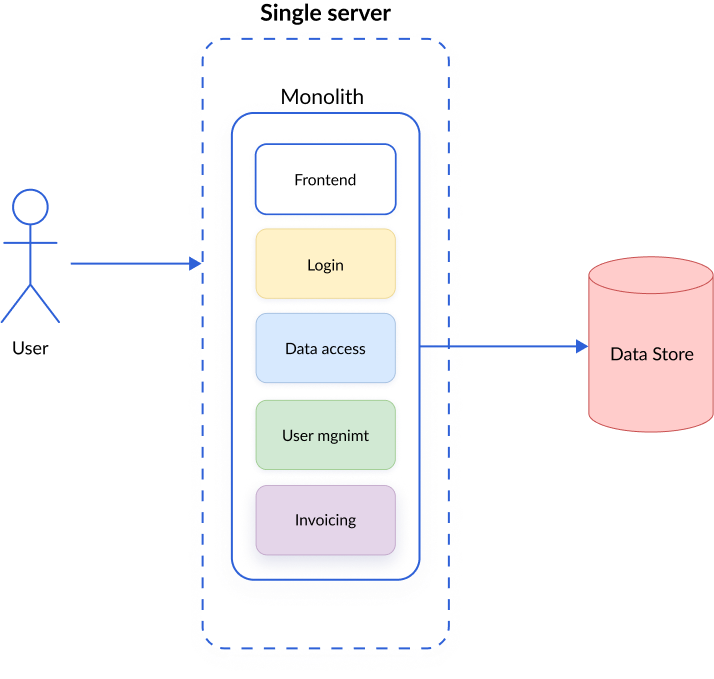
\includegraphics[width=.7\textwidth]{graphics/img/mono.png}
  \caption{Пример монолитной архитектуры}
  \label{fig:mono}
\end{figure}


Микросервисная архитектура - это разделение архитектуры на множество независимо функционирующих служб. Каждая из этих служб имеет свою бизнес-логику и систему управления базами данных (СУБД), служащую определенной цели. Оба эти типа архитектур стоит рассмотреть в контексте сравнения.

\begin{figure}
  \centering
  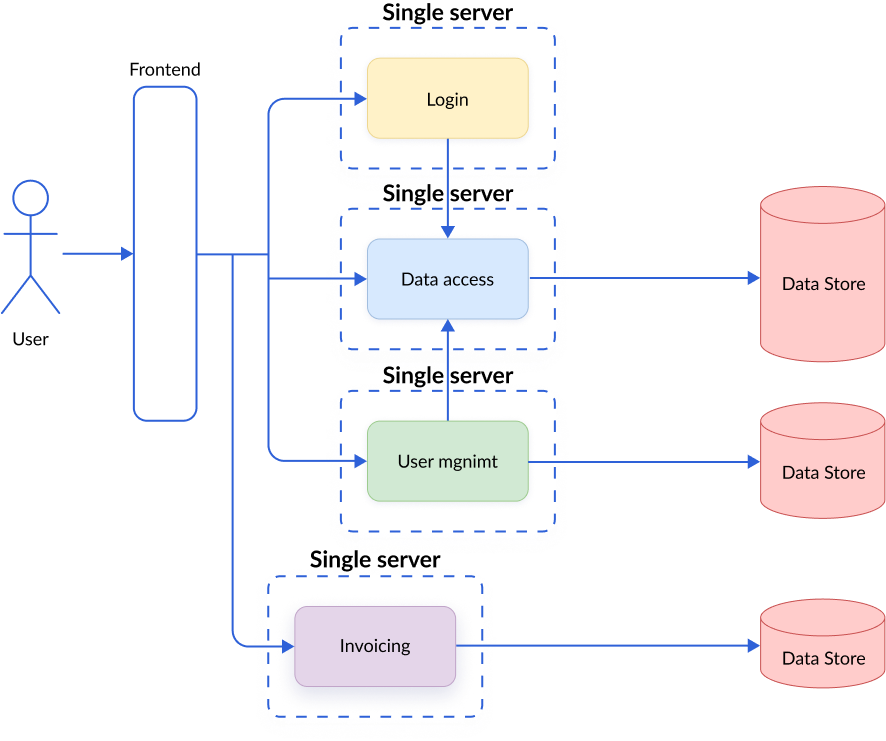
\includegraphics[width=.9\textwidth]{graphics/img/micro.png}
  \caption{Пример микросервисной архитектуры}
  \label{fig:micro}
\end{figure}

Среди недостатков монолитной архитектуры можно выделить плохую масштабируемость, трудность внедрения новых модулей и проблемы при обновлении технологий, так как это может затронуть весь проект, к тому же есть и проблемы с отказоустойчивостью и трудностью в горизонтальной масштабируемости. Однако она проще в развертывании, разработке, тестировании и отладке, чем микросервисная. \cite{arch:monovsmicro}

Микросервисная архитектура обладает гибкостью: каждая команда может разрабатывать и разворачивать свой сервис независимо, что ускоряет сроки реализации проектов и позволяет выбирать технологии согласно предпочтениям команды. Отказоустойчивость в данном случае - тоже немаловажный плюс, поскольку при сбое одного микросервиса функциональность приложения страдает лишь частично. Недостатками же можно считать большие затраты при разрастании приложения и сложность отладки и координации между разными командами.

Текущий проект работы подразумевает под собой максимальную нагрузку, портируемость и отказоустойчивость. С учетом этого, было решено использовать микросервисную архитектуру, да и существующие системы неспроста являются микросервисными, так как высокие требования делают зависимость от более гибкой системы.

\section{Функциональные возможности системы}

Выробатанными требованиями мы приходим к функциональным возможностям проектируемой системы:

\subsection{Серверная часть системы}

Серверная часть системы должна обладать данными функциональными возможностями, такими как:

\begin{enumerate}
    \item Загрузка на сервер, отправка пакета (модуля) с сервера.
    \item Управление зависимостями модулей.
    \item Система версий модулей.
    \item Информирование о модулях и их безопасности.
    \item Аутефикация и авторизация на основе JWT.
    \item Реализация открытого API.
    \item Система блокировки и защиты особо критических модулей.
\end{enumerate}

\Abbrev{API}{Application Programming Interface}

\Define{API}{Application Programming Interface ""--- представляет собой набор правил и инструкций, согласно которым различные программы и сервисы могут общаться между собой. Эти правила определяют, как данные и функциональность могут быть переданы от одной программы к другой, как они могут взаимодействовать и обмениваться информацией}

\subsection{Клиентская часть системы}

Клиентская часть системы должна обладать данными функциональными возможностями, такими как:

\begin{enumerate}
    \item Простой и понятный интерфейс через CLI.
    \item Конфигурирование клиентской части.
    \item Управление установленными модулями, включая загрузку, обновление и удаление.
    \item Информирование о модулях и их безопасности.
\end{enumerate}

\section{Микросервис авторизации}

В предложенной работе необходимо разработать микросервис авторизации для системы. Он будет отвечать за следующие функции: 

\begin{enumerate}
    \item регистрацию пользователя.
    \item аутентификацию и авторизацию пользователя.
    \item система сессий через JWT.
    \item система прав у пользователей.
\end{enumerate}

\begin{figure}
  \centering
  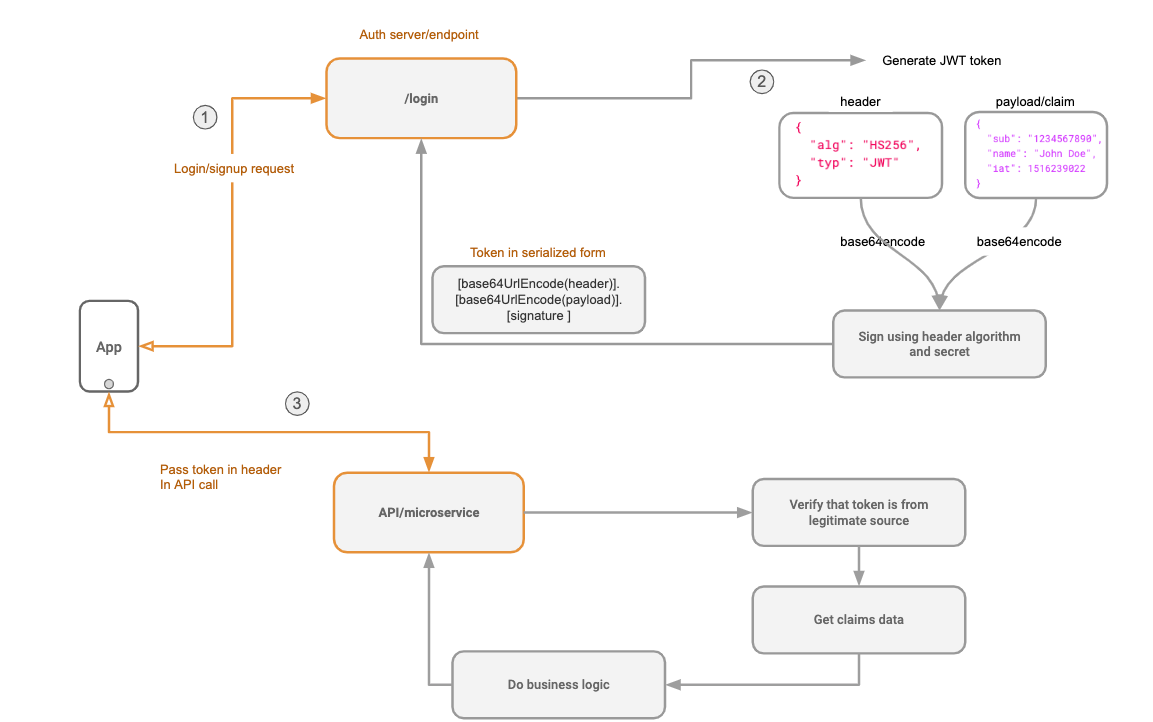
\includegraphics[width=0.8\textwidth]{graphics/img/jwt.png}
  \caption{Функционирование JWT в связке клиент-сервер}
  \label{fig:jwt}
\end{figure}

\Abbrev{JWT}{JSON Web Token}
\Define{JWT}{JSON Web Token ""--- руководствующийся открытым стандартом (RFC 7519), представляет собой универсальное средство формирования токенов доступа, рснованный на надежном и широкораспространенном формате JSON, он стал одним из наиболее эффективных и безопасных способов обеспечения эффективной передачи информации между устройствами и серверами в кодированном виде}

\section{API Gateway}
Для полноценного функционирования и получения доступка к микросервисам из любой точки Интернета, необходима единая точка входа, называемая API Gatawey, в качестве которого будет выступать прокси сервер nginx, с модулем поддержки JWT. \cite{arch:api}
\begin{enumerate}
    \item проксирование на необходимые микросервисы;
    \item балансировка нагрузки на запущенные микросервисы;
    \item проверка и прочие действия с JWT;
    \item реализация всех современных стандартов безопасности (CORS и прочие механизмы);
\end{enumerate}

\Define{nginx}{это HTTP-сервер и обратный прокси-сервер, почтовый прокси-сервер, а также TCP/UDP прокси-сервер общего назначения, изначально написанный Игорем Сысоевым}

\Define{CORS-заголовки}{(Cross-Origin Resource Sharing) ""--- это механизм веб-безопасности, который позволяет браузеру загружать данные из стороннего интернет-источника.}

\Define{API Gatawey}{шлюз для API, который упрощает их управление и делает их доступными для клиентов.}

Таким образом, только API Gateway и микросервис авторизации имеют доступ к единому хранилищу, где располагается секретный ключ, используемый для подписи JWT, что повышает безопасность системы в целом. Для предовращения и снижения риска компроментации, ключ рекомендуется менять раз в месяц. 

\section{Микросервис управления пакетами}

Микросервис управления модулями является основным и включает в себя ряд функций и способностей. 

\subsection{Базовый функционал}
Сервис обеспечивает добавление новых модулей, управление их распределением и поиск по модулям в соответствии с запросами пользователя.

\subsection{Система зависимостей}
Сервис предоставляет возможность модулям иметь систему зависимостей, что позволяет создавать модульные приложения и пакеты.

\subsection{Блокировка, поиск уязвимостей и удаление модулей}
Ключевую роль в функционале микросервиса играет возможность блокировки модулей, что является важным средством контроля доступа. Кроме того, микросервис может производить поиск и устранение уязвимостей в модулях, что особенно важно с точки зрения безопасности системы.

\subsection{Информирование}
Функция информирования обеспечивает прозрачность и контроль над процессами управления модулями. С помощью неё пользователи могут получать обновленную информацию о статусе операций и о состоянии модулей.

\section{CDN}

\Abbrev{CDN}{Content Delivery Network}
\Define{CDN}{Content Delivery Network ""--- это сеть распределенных серверов, которые эффективно передают контент пользователям, основываясь на их географическом положении, источнике контента и сервере с оригинальным содержимым}

В контексте проектирования системы, CDN обеспечивает надежную, высокоскоростную и эффективную доставку модулей от сервера к клиенту. Благодаря CDN, пакеты кода или модулей могут быть быстро и эффективно переданы пользователям независимо от их географического расположения.

\begin{figure}
  \centering
  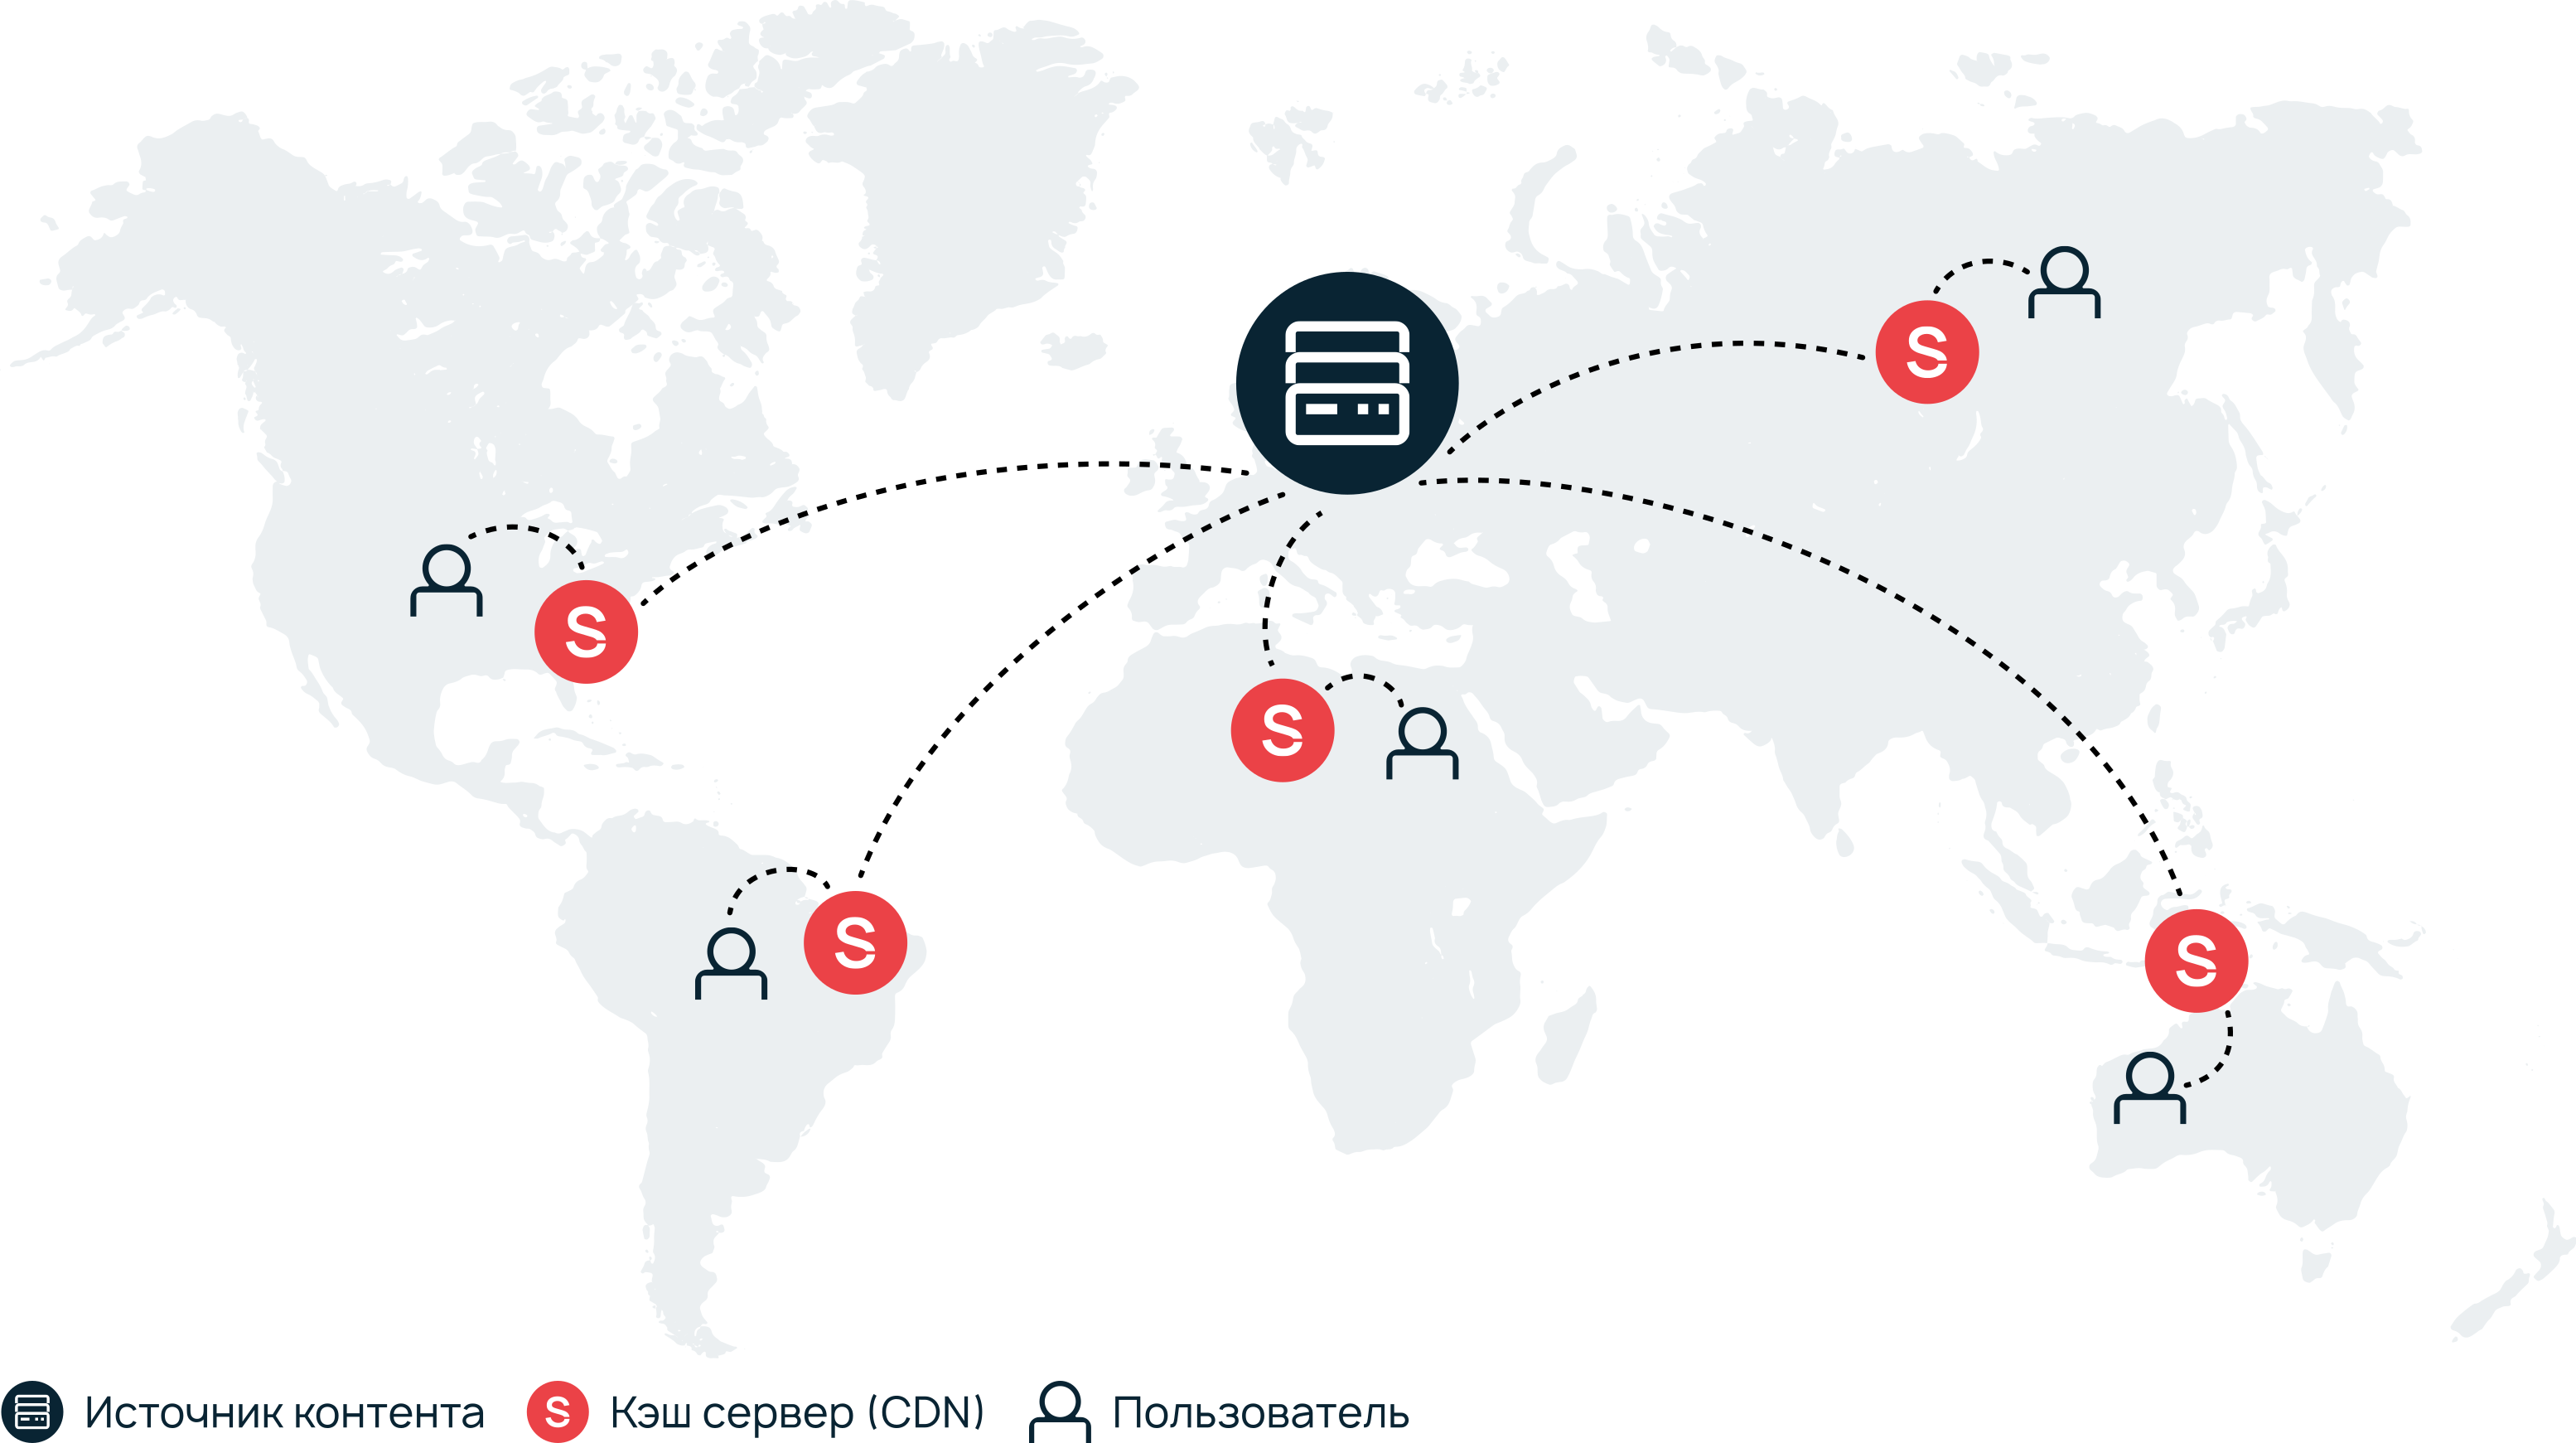
\includegraphics[width=.8\textwidth]{graphics/img/sheme-cdn}
  \caption{Пример визуализации работы CDN}
  \label{fig:mono}
\end{figure}

Когда разработчик выдает команду для установки определенного модуля, клиент обращается к своему реестру (образу базы данных всех доступных модулей), который размещен в CDN.

Работая в совокупности с CDN, система дистрибрюции осуществляет следующие функции:

\begin{enumerate}
    \item Обеспечивает надежную и быструю доставку пакетов на компьютеры разработчиков.
    \item Снижает задержку в сети благодаря географическому размещению серверов CDN ближе к пользователям.
    \item Обеспечивает глобальное масштабирование, так как CDN может эффективно обслуживать тысячи запросов по всей России в разных частях и всему миру.
    \item Увеличивает отказоустойчивость и распределенность системы, поскольку множество точек присутствия CDN могут обслуживать запросы в случае отказа какой-либо из них.
    \item Снижает нагрузку на основные сервисы за счет кеширования.
\end{enumerate}

 При проектировании я решил использовать услуги отечественного провайдера CDN компании Selectel. \cite{cdn:selectel} Выбор данного провайдера был сделан на основе ряда преимуществ, которые он предлагает.

Selectel предоставляет надежные CDN-услуги, что значительно ускоряет загрузку контента, где бы пользователь не находился. Это особенно важно для нашего проекта, так как ориентир на географически распределенную аудиторию и нуждаемся в том, чтобы модули доставлялись быстро и надежно.

Компания обеспечивает высокую доступность пакетов из-за использования глобальной сети серверов внутри России и по всему миру.

При этом зона собственного покрытия CDN Selectel включает себя такие города \cite{cdn:selectel}, как:
\begin{itemize}
    \item Россия: Барнаул, Владивосток, Екатеринбург, Иркутск, Казань, Кемерово, Кизляр, Краснодар, Красноярск, Москва, Новосибирск, Орел, Ростов-на-Дону, Санкт-Петербург, Самара, Симферополь, Уфа, Хабаровск, Южно-Сахалинск
    \item Азия: Алматы, Бишкек, Гонконг, Сингапур, Ташкент
    \item Америка: Ашберн, Сан-Паулу
    \item Европа: Амстердам, Минск, Сухум, Франкфурт
\end{itemize}

\begin{figure}
  \centering
  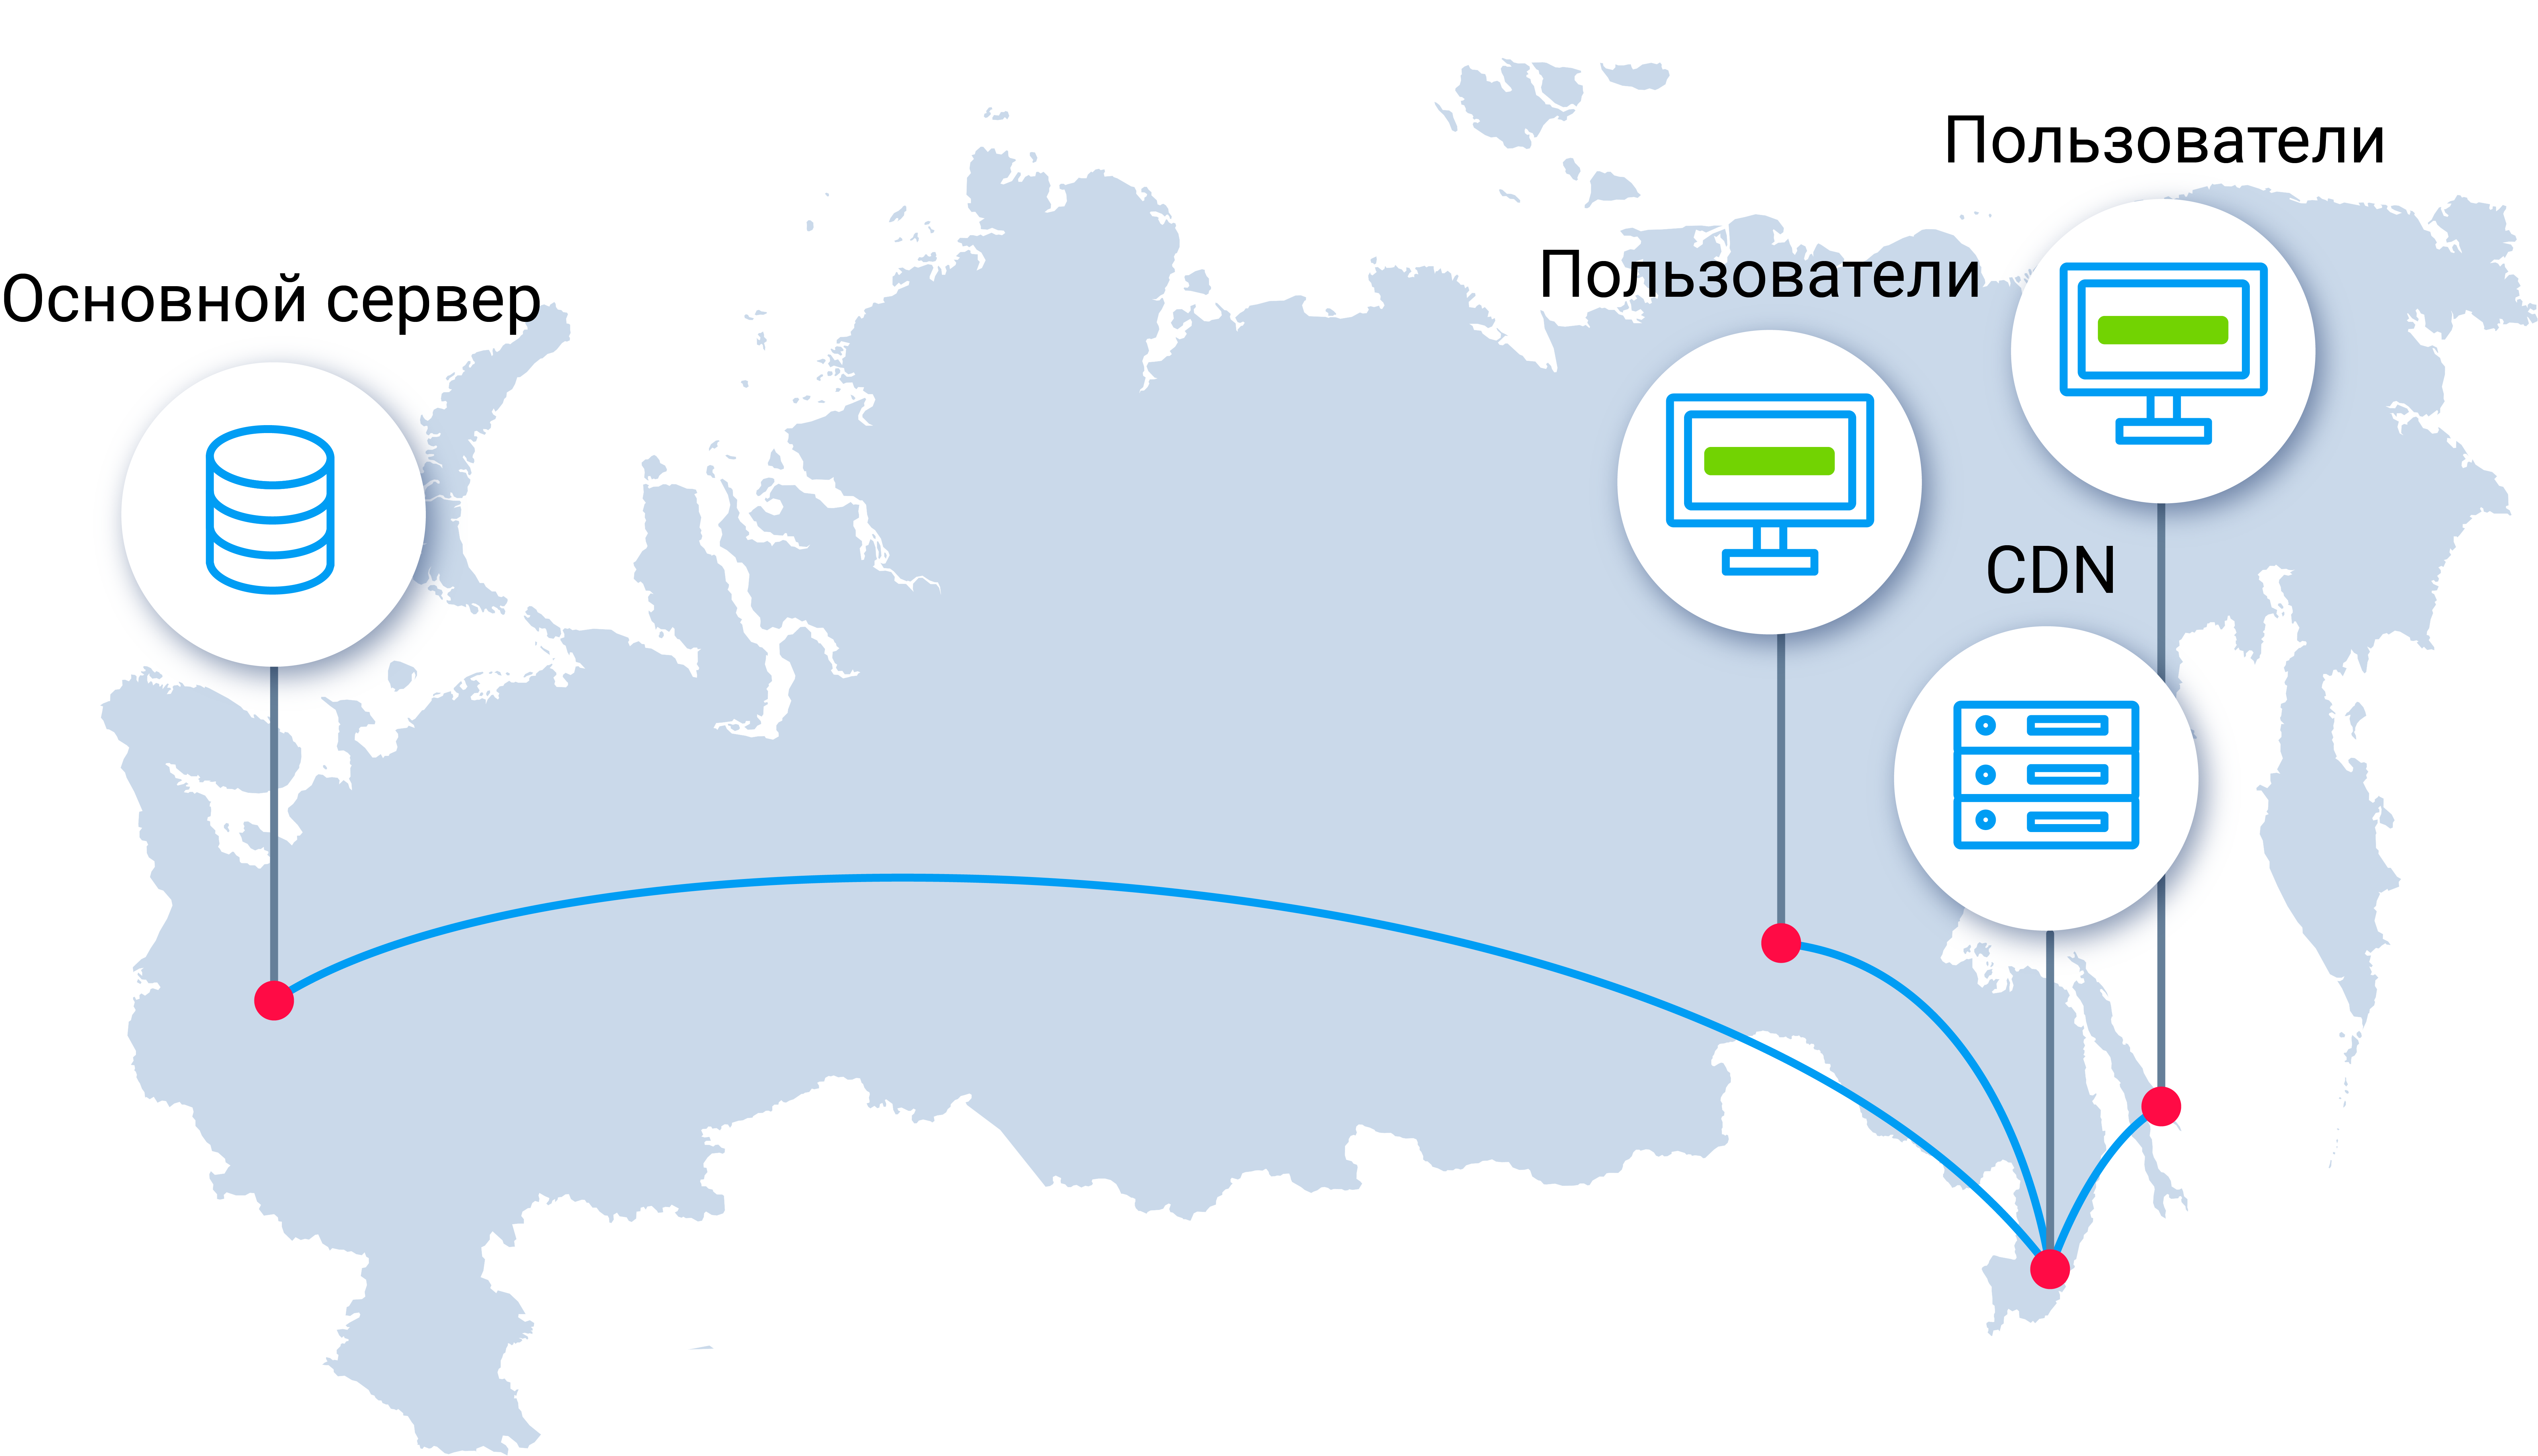
\includegraphics[width=.8\textwidth]{graphics/img/cdn.scheme.5Y4Ydf}
  \caption{Пример визуализации работы CDN в рамках России}
  \label{fig:cdn_russia}
\end{figure}

Это увеличивает отказоустойчивость проекта и позволяет нам быть уверенными в постоянной доступности модулей для пользователей.

Серверы Selectel обладают высокой пропускной способностью, что среднее время отлика составляет 30 милисекунд \cite{cdn:selectel}, что обеспечивает максимальную скорость передачи данных. Это особенно ценно для системы модульного менеджера, поскольку она имеет дело с большим количеством пакетов, которые должны быть быстро доставлены пользователям.

Кроме того, Selectel уделяет особое внимание вопросам безопасности и защиты данных. Наши пакеты и пользовательские данные хранятся с учетом последних стандартов безопасности, и мы можем быть уверенны в их надежности и защищенности.

При работе с отечественным провайдером у нас также есть возможность получить более оперативную техническую поддержку и консультации по связанным вопросам, что значительно упрощает процесс взаимодействия и решения возникающих вопросов.

В целом, CDN как он встроен в систему, является одним из ключевых факторов обеспечения эффективной и надежной доставки пакетов и модулей, а использование услуг CDN от Selectel, обеспечивает надежность, высокую скорость доставки пакетов, а также высокую степень безопасности данных, что ускоряет время развертывания и обновления проектов, но и снижает время простоя, повышая общую производительность и эффективность процесса разработки ПО.

\section{Оборудование и ОС как часть системы}

Учитывая связанные риски и выроботонные с этим направления, при проектировании необходимо создать решение, совместимое с российским процессором компании МЦСТ, именованный «Эльбрус-8СВ».

Эльбрус-8СВ - является восьмиядерным промышленным процессором на базе архитектуры Эльбрус (e2k) с использованием длинного командного слова (VLIW), разработанным в России. Он создан для работы в 64-разрядной вычислительной системе и может обрабатывать до 288 гигафлопс двойной точности в одноядерном режиме при частоте 1.5 ГГц, будучи произведенным по техническим нормам в 28 нанометров. 

\Define{Гигафлопс}{Индикатор, определяющий скорость работы суперкомпьютера. 1 г= 109 aial/s, т. е. суперкомпьютер 1 сек.в 1 млрд. выполняет арифметические и логические операции.}

\Abbrev{VLIW}{Very Long Instruction Word}
\Define{VLIW}{Very Long Instruction Word ""--- архитектура процессоров с несколькими вычислительными устройствами. Характеризуется тем, что одна инструкция процессора содержит несколько операций, которые должны выполняться параллельно. Фактически это «видимое программисту» микропрограммное управление, когда машинный код представляет собой лишь немного свёрнутый микрокод для непосредственного управления аппаратурой}

Ключевым преимуществом Эльбруса является его отечественное происхождение, что даёт возможность избегать определенных проблем и рисков, связанных с использованием процессоров Intel и AMD. При этом, параметры процессора позволяют полностью закрыть вопрос в потребностях сервисов.

\begin{figure}
  \centering
  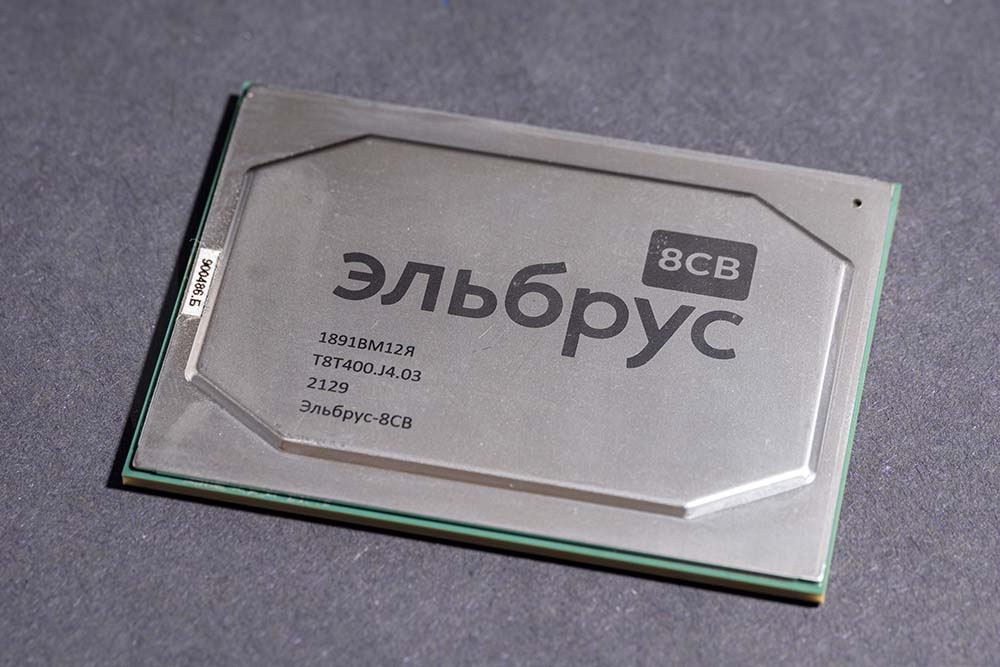
\includegraphics[width=.6\textwidth]{graphics/img/elbrus}
  \caption{Внешний вид процессора компании МЦСТ - Эльбрус-8СВ}
  \label{fig:elbrus}
\end{figure}

В свете недавних проблем с безопасностью в процессорах Intel и AMD, таких как утечка данных через атаки Spectre и Meltdown, проблемы с микрокодом и другие, использование процессора Эльбрус представляет собой весьма привлекательное решение. Он обладает потенциалом минимизировать тактические и стратегические риски связанные с используемым железом, включая риски иностранных поставок, уязвимости безопасности и ответственность за продукт.

Атаки Spectre и Meltdown стали известны в 2018 году и поставили под угрозу безопасность процессоров Intel, ARM, AMD и некоторых других. Эти атаки используют уязвимости в методах оптимизации работы процессора — так называемой спекулятивной и предсказательной вычислительной системе.

Meltdown и Spectre эксплуатируют «спекулятивное выполнение» \cite{risk:spectual_hack} - функцию, при которой процессор предварительно вырабатывает инструкции, которые могут понадобиться в дальнейшем, чтобы ускорить выполнение кода. Это делает системы уязвимыми, поскольку атакующие могут гипотетически пройти по этим предварительным вычислениями и получить доступ к конфиденциальной информации, которую обычно не должны были бы видеть.

Внедрение исправлений для этих уязвимостей в микрокод процессоров Intel и AMD столкнулось с рядом проблем. Например, первоначальные исправления от Intel вызвали проблемы с перезагрузкой и привели к снижению производительности у некоторых пользователей. Затем Intel выпустил обновленные патчи, чтобы решить эти проблемы. AMD также столкнулась с проблемами, связанными с исправлениями Spectre, но в конечном итоге выпустила серию обновлений микрокода для устранения этих уязвимостей.

\Abbrev{Intel ME}{Intel Management Engine}
При этом, Intel ME, это встроенный модуль микроконтроллера, присутствующий во всех чипсетах Intel с 2006 года, который имеет полный доступ к памяти компьютера, сети и другим частям системы, даже когда компьютер выключен или система спит.

Аналогом Intel Management Engine в мире AMD является AMD Secure Technology, которую ранее называли Secure Processor (или Platform Security Processor, PSP). PSP от AMD также был подвержен уязвимости, схожей у Intel ME \cite{risk:amdpsp}.

Уязвимости Intel ME представляют собой нарушение безопасности из-за незадокументированных возможностей данной части процессора, с возможностью удаленно управлять и исполнять код внутри Intel ME, что и демострируют специалисты компании Positive Technologies \cite{risk:intelme}, показывая возможность выполнения кода даже на выключенном сервере. Эти уязвимости позволяют хакерам возиться с компьютером, обходя встроенные защитные механизмы. По сути, это означает, что злоумышленник может полностью контролировать компьютер с уязвимостью Intel ME, управлять его работой и получать доступ к любым его данным.

Для управления используется AMT, который работает постоянно, жесткий диск — нет, но для изменения кода в  Intel ME жесткого диска не нужен. При этом, обычное ожидание ничем не дает безопасности. При этом у Intel есть технология конфигурации с другого хоста, можно в качестве другого хоста подсунуть взломанный Intel ME, и он заразит соседний сервер в результате, а все сервера «выключены». Аппаратные возможности таких решений настараживают и заставляют отказаться от данных процессоров этих компаний.

Однако российские процессоры Эльбрус не были уязвимы для этих атак. Это объясняется архитектурой и методами оптимизации работы процессора, отличающимися от используемых в Intel и AMD. Конкретно, процессоры «Эльбрус» не используют подобное спекулятивное выполнение и системы управления процессором, а значит, уязвимые атаки не могут быть использованы. \cite{risk:elbrus_no_spectre}

В качестве оптимальной операционной системы, которую можно реализовать на оборудовании Эльбрус с использованием пакетного менеджера, можно рассматривать AstraLinux. Это российский дистрибутив на основе Debian GNU/Linux, который нацелен на создание унифицированной, безопасной и легко управляемой операционной системы, c обеспечением высоким уровенем защиты, что особенно важно при работе с критической инфраструктурой, такие как системы дистрибюции модулей.


%%% Local Variables:
%%% mode: latex
%%% TeX-master: "rpz"
%%% End:

\chapter{Технологический раздел}
\label{cha:impl}

В данном разделе описано изготовление и требование всячины. Кстати,
в Latex нужно эскейпить подчёркивание (писать <<\verb|some\_function|>> для \Code{some\_function}).

\ifPDFTeX
Для вставки кода есть пакет \Code{listings}. К сожалению, пакет \Code{listings} всё ещё
работает криво при появлении в листинге русских букв и кодировке исходников utf-8.
В данном примере он (увы) на лету конвертируется в koi-8 в ходе сборки pdf.

Есть альтернатива \Code{listingsutf8}, однако она работает лишь с
\Code{\textbackslash{}lstinputlisting}, но не с окружением \Code{\textbackslash{}lstlisting}

Вот так можно вставлять псевдокод (питоноподобный язык определен в \Code{listings.inc.tex}):

\begin{lstlisting}[style=pseudocode,caption={Алгоритм оценки дипломных работ}]
def EvaluateDiplomas():
    for each student in Masters:
        student.Mark := 5
    for each student in Engineers:
        if Good(student):
            student.Mark := 5
        else:
            student.Mark := 4
\end{lstlisting}

Еще в шаблоне определен псевдоязык для BNF:

\begin{lstlisting}[style=grammar,basicstyle=\small,caption={Грамматика}]
  ifstmt -> "if" "(" expression ")" stmt |
            "if" "(" expression ")" stmt1 "else" stmt2
  number -> digit digit*
\end{lstlisting}

В листинге~\ref{lst:sample01} работают русские буквы. Сильная магия. Однако, работает
только во включаемых файлах, прямо в \TeX{} нельзя.

% Обратите внимание, что включается не ../src/..., а inc/src/...
% В Makefile есть соответствующее правило для inc/src/*,
% которое копирует исходные файлы из ../src и конвертирует из UTF-8 в KOI8-R.
% Кстати, поэтому использовать можно только русские буквы и ASCII,
% весь остальной UTF-8 вроде CJK и египетских иероглифов -- нельзя.

\lstinputlisting[language=C,caption=Пример (\Code{test.c}),label=lst:sample01]{inc/src/test.c}

\else

Для вставки кода есть пакет \texttt{minted}. Он хорош всем кроме: необходимости Python (есть во всех нормальных (нет, Windows, я не про тебя) ОС) и Pygments и того, что нормально работает лишь в \XeLaTeX.

\ifdefined\NoMinted
Но к сожалению, у вас, по-видимому, не установлен Python или pygmentize.
\else
Можно пользоваться расширенным BFN:

\begin{listing}[H]
\begin{ebnfcode}
 letter = "A" | "B" | "C" | "D" | "E" | "F" | "G"
       | "H" | "I" | "J" | "K" | "L" | "M" | "N"
       | "O" | "P" | "Q" | "R" | "S" | "T" | "U"
       | "V" | "W" | "X" | "Y" | "Z" ;
digit = "0" | "1" | "2" | "3" | "4" | "5" | "6" | "7" | "8" | "9" ;
symbol = "[" | "]" | "{" | "}" | "(" | ")" | "<" | ">"
       | "'" | '"' | "=" | "|" | "." | "," | ";" ;
character = letter | digit | symbol | "_" ;
 
identifier = letter , { letter | digit | "_" } ;
terminal = "'" , character , { character } , "'" 
         | '"' , character , { character } , '"' ;
 
lhs = identifier ;
rhs = identifier
     | terminal
     | "[" , rhs , "]"
     | "{" , rhs , "}"
     | "(" , rhs , ")"
     | rhs , "|" , rhs
     | rhs , "," , rhs ;
 
rule = lhs , "=" , rhs , ";" ;
grammar = { rule } ;
\end{ebnfcode}
\caption{EBNF определённый через EBNF}
\label{lst:ebnf}
\end{listing}

А вот в листинге \ref{lst:c} на языке C работают русские комменты. Спасибо Pygments и Minted за это.

\begin{listing}[H]
\cfile{lyx/inc/src/test.c}
\caption{Пример — test.c} 
\end{listing}
\label{lst:c}

\fi
\fi
% Для вставки реального кода лучше использовать \texttt{\textbackslash lstinputlisting} (который понимает
% UTF8) и стили \Code{realcode} либо \Code{simplecode} (в зависимости от размера куска).




Можно также использовать окружение \Code{verbatim}, если \Code{listings} чем-то не
устраивает. Только следует помнить, что табы в нём <<съедаются>>. Существует так же команда \Code{\textbackslash{}verbatiminput} для вставки файла.

\begin{verbatim}
a_b = a + b; // русский комментарий
if (a_b > 0)
    a_b = 0;
\end{verbatim}

%%% Local Variables:
%%% mode: latex
%%% TeX-master: "rpz"
%%% End:

\chapter{Тестирование}
\label{cha:research}

Запустим сервер командой sakurajima-server

\begin{figure}
  \centering
  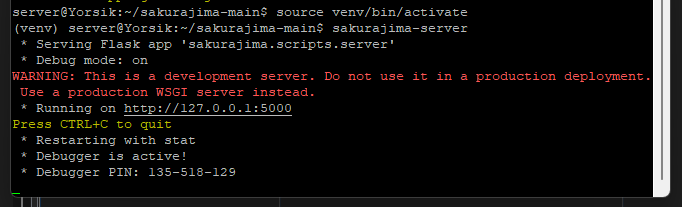
\includegraphics[width=.9\textwidth]{graphics/test/dev_server_run.png}
  \caption{Демонстрация информации о статусе запуска сервера (Flask)}
  \label{fig:test1}
\end{figure}

Проведем тестирование заявленного функционала:

\begin{enumerate}

\item Справка по командам


\item Авторизация и аутификация


\item Создание модуля

Для создания модуля следует создать папку с названием соответствующего модуля в нужном месте. Внутри этой папки следует разместить файл module.json, в котором указываются имя и версия модуля. Возьмем для примера модуль с названием demo версии 1.0.0.

\begin{figure}
  \centering
  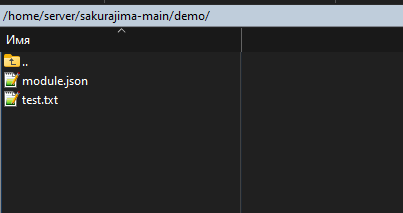
\includegraphics[width=.6\textwidth]{graphics/test/demo_r.png}
  \caption{Содержимое папки модуля demo}
  \label{fig:test1}
\end{figure}
\newpage
    \item Отправка модуля

Впоследствии, выполняем команду sakurajima upload demo, которая загружает модуль под названием demo на сервер.

\begin{figure}
  \centering
  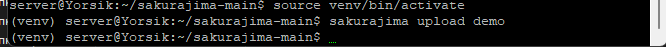
\includegraphics[width=1.0\textwidth]{graphics/test/demo.png}
  \caption{Выполнение команды отправки модуля на сервер в CLI}
  \label{fig:test1}
\end{figure}

В итоге, на сервере появляется конкретная версия модуля и последняя версия.

\begin{figure}
  \centering
  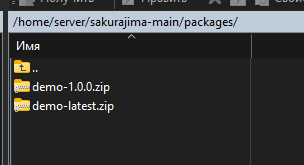
\includegraphics[width=.7\textwidth]{graphics/test/demo_alias_modules.png}
  \caption{Содержимое папки модулей на сервере}
  \label{fig:test1}
\end{figure}

\item Обновление модуля

Модифицируем версию модуля в файле и добавляем дополнительный файл - изображение. Затем повторно активизируем команду sakurajima upload demo.

\begin{figure}
  \centering
  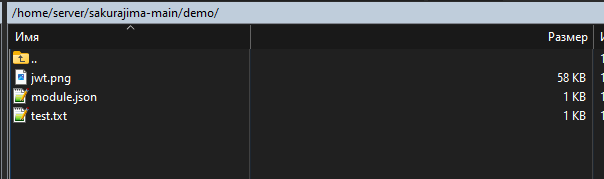
\includegraphics[width=.8\textwidth]{graphics/test/demo_jwt.png}
  \caption{Обновленное содержимое папки модуля demo}
  \label{fig:test1}
\end{figure}

\newpage

Теперь у нас имеется две версии - 1.0.0 и 1.5.0.

\begin{figure}
  \centering
  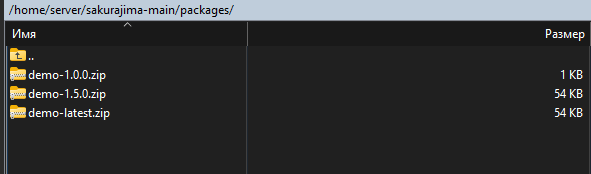
\includegraphics[width=.8\textwidth]{graphics/test/demo_jwt_final.png}
  \caption{Обновленное содержимое папки модулей на сервере}
  \label{fig:test1}
\end{figure}

\item Загрузка модуля

Для проверки функционирования загрузки модуля demo, предварительно удалим локально.

Используем следующую команду: sakurajima install name-module==version

Стандартная процедура установки предусматривает установку самой последней версии модуля (latest).

\begin{figure}
  \centering
  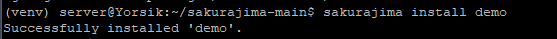
\includegraphics[width=.8\textwidth]{graphics/test/dev_install.png}
  \caption{Результат выполнения команды установки модуля demo}
  \label{fig:test1}
\end{figure}

Если мы укажем через `==` версия, то будет загружена определенная версия модуля.

\begin{figure}
  \centering
  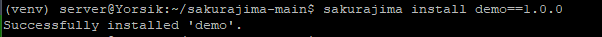
\includegraphics[width=.8\textwidth]{graphics/test/dev_install_ver.png}
  \caption{Результат выполнения команды установки модуля demo с конкретной версией}
  \label{fig:test1}
\end{figure}

\newpage

\item Удаление модуля

Используем команду: sakurajima uninstall name-module

\begin{figure}
  \centering
  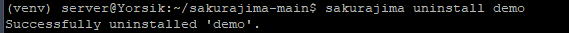
\includegraphics[width=.8\textwidth]{graphics/test/dev_uninstall.png}
  \caption{Результат выполнения команды удаления модуля demo}
  \label{fig:test1}
\end{figure}

\item Проверка модуля на увязвимости

Используем команду: sakurajima cve

\item Система зависимостей в модулях

\begin{figure}
  \centering
  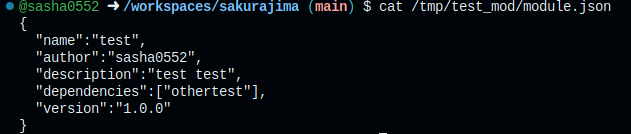
\includegraphics[width=.8\textwidth]{graphics/test/info2.png}
  \caption{Содержимое тестового модуля с указанием зависимостей (dependencies)}
  \label{fig:test1}
\end{figure}

\item Информирование о модуле

Используем команду: sakurajima info

\begin{figure}
  \centering
  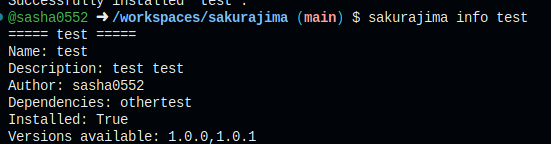
\includegraphics[width=.8\textwidth]{graphics/test/info3.png}
  \caption{Результат команды для установленного локально модуля}
  \label{fig:test1}
\end{figure}


\end{enumerate}

%%% Local Variables:
%%% mode: latex
%%% TeX-master: "rpz"
%%% End:

\chapter{Организационно-экономический раздел}
\label{cha:econom}

\section{Протестируем специальные символы.}

И заодно переключение шрифтов.


{\shorthandoff" \texttt{"-{}-* Прямая речь "-{}-{}- <{}<после ,{},тире`{}` неразрывный пробел>{}>}}

{\cyrillicfonttt{\bfseries\itshape\textbackslash{}cyrillicfonttt}
"--* Прямая речь "--- <<после ,,тире`` неразрывный пробел>>.}

{\cyrillicfontsf{\bfseries\itshape\textbackslash{}cyrillicfontsf}
"--* Прямая речь "--- <<после ,,тире`` неразрывный пробел>>.}

{\cyrillicfont{\bfseries\itshape\textbackslash{}cyrillicfont}
"--* Прямая речь "--- <<после ,,тире`` неразрывный пробел>>.}


%%% Local Variables:
%%% mode: latex
%%% TeX-master: "rpz"
%%% End:


\backmatter %% Здесь заканчивается нумерованная часть документа и начинаются ссылки и
            
\Conclusion % заключение к отчёту

В результате проделанной работы были полученны данные результаты:

\begin{enumerate}
    \item Мировой опыт в области систем был изучен, проанализированы преимущества и недостатки, а также потенциальные риски.
    \item Определены функциональные требования к создаваемому сервису, на основе которых были спроектированы и реализованы два независимых микросервиса, отвечающих за аутентификацию и управление пакетами.
    \item Спроектирован проект, в ходе которого была разработана система распределения модулей.
    \item Отбраны российские решения для интеграции во свою систему, чтобы избежать зависимости от иностранной инфраструктуры.
    \item Реализовано минималистичное приложение с клиентской стороны в формате CLI, предлагающее простой и удобный интерфейс для управления модулями.
    \item Реализовано серверное приложение, предоставляющее возможности управления модулями, включая системы анализа безопасности.
\end{enumerate}

\newpage
За время выполнения курсовой работы были реализованы следующие компетенции:
\begin{table}[h!]
\centering
\begin{tabular}{|p{3cm}|p{5cm}|p{7cm}|} 
    \hline
    Шифр \newline компетенции & Расшифровка \newline приобретаемой \newline компетенции & Расшифровка освоения \newline компетенции \\[0.5ex] 
        \hline
        УК-6 & Способен управлять своим временем, выстраивать и реализовывать траекторию саморазвития на основе принципов образования в течение всей жизни &  Процесс реализации системы был разбит по шагам, которые выполнялись в отведенное для них время, включая отдельно поэтапное время на изучение.  \\ \hline
        ПК-4 & Разработка требований и проектирование программного обеспечения & Проанализирована тщательно ситуация на рынке систем с учетом текущей ситуации и выработаны требования к системе. \\  \hline
        ПК-5 & Оценка и выбор варианта архитектуры программного средства & Был проведен изучение существующих решений, а так-же выработаны из требований условия функционирования системы, что в результате превратилось в клиент-серверную, где сервер использует микросервесную архитектуру. \\  \hline
        ПК-6 & Разработка тестовых случаев, проведение тестирования и исследование результатов & Проведен полный комплекс тестов, потвердивших работоспособность всей системы, начиная от проектирования и вплоть до разработки.\\ 
 \hline
\end{tabular}
\caption{Компетенции при выполнении курсовой работы}
\label{table:1}
\end{table}

%%% Local Variables: 
%%% mode: latex
%%% TeX-master: "rpz"
%%% End: 
%% заключение


% % Список литературы при помощи BibTeX
% Юзать так:
%
% pdflatex rpz
% bibtex rpz
% pdflatex rpz


\bibliographystyle{ugost2008}
\bibliography{rpz}

%%% Local Variables: 
%%% mode: bibtex
%%% TeX-master: "rpz"
%%% End: 



\appendix   % Тут идут приложения

\chapter{Картинки}
\label{cha:appendix1}

\begin{figure}
\centering
\caption{Картинка в приложении. Страшная и ужасная.}
\end{figure}

%%% Local Variables: 
%%% mode: latex
%%% TeX-master: "rpz"
%%% End: 


\chapter{Еще картинки}
\label{cha:appendix2}
\blindtext

\begin{figure}
\centering
\caption{Еще одна картинка, ничем не лучше предыдущей. Но надо же как-то заполнить место.}
\end{figure}

%%% Local Variables: 
%%% mode: latex
%%% TeX-master: "rpz"
%%% End: 


\end{document}

%%% Local Variables:
%%% mode: latex
%%% TeX-master: t
%%% End:
